\section{VHDL-Programmierung}

\subsection{Vorgefertigte Module}

\begin{frame}
	\frametitle{VHDL-Programierung}
	\framesubtitle{Hardwareabstraktion im Detail}
	\begin{beamerboxesrounded}{Vorgefertigte Module: Abstraktionmodule}
		\begin{itemize}[<+->]
			\item Initialisierungmodul
			\item Takterzeugung
			\item AD- bzw. DA-Umsetzer ($I^2S$-Schnittstelle $\Rightarrow$ parallel)
			\item Vorverst�rkerregelung
			\item 7-Segmentdecoder
			\item Mikrofonvorverst�rkerregelung
			\item Pegelanzeige-Abstraktion
			\item Schalter-/Tasterentprellung
		\end{itemize}
	\end{beamerboxesrounded}	
\end{frame}

\subsection{Musterl�sungen}

\begin{frame}
	\frametitle{VHDL-Programierung}
	\framesubtitle{Hardwareabstraktion im Detail}
	\begin{beamerboxesrounded}{Studentische Module: Musterl�sungen}
		\begin{itemize}[<+->]
			\item Erste Schritte: Multiplexer
			\item (Pseudo-)Zufallszahlengenerator
			\item Signalgenerator
			\item Pegelanzeige (f�r Fehlersuche)
			\item Modulator
			\item Bandpass (Suboptimal)
			\item Bandpass (Optimal)
			\item Demodulator
			\item Tiefpass
			\item Signalregenerierung (Hysterese)
			\item Zusammenschaltung
		\end{itemize}
	\end{beamerboxesrounded}	
\end{frame}

\subsection{Verfikation}

\begin{frame}
	\frametitle{VHDL-Programierung}
	\framesubtitle{Verifiaktion: Testbenches}
	\begin{beamerboxesrounded}{Verifikation}
		\begin{itemize}
			\item Alle Module wurden verifiziert
			\item K�nnen den Studenten als Verifikation dienen
		\end{itemize}
	\end{beamerboxesrounded}
	\begin{beamerboxesrounded}{Beispiel: Bandpass (optimal)}
		\begin{center}
			\begin{figure}
				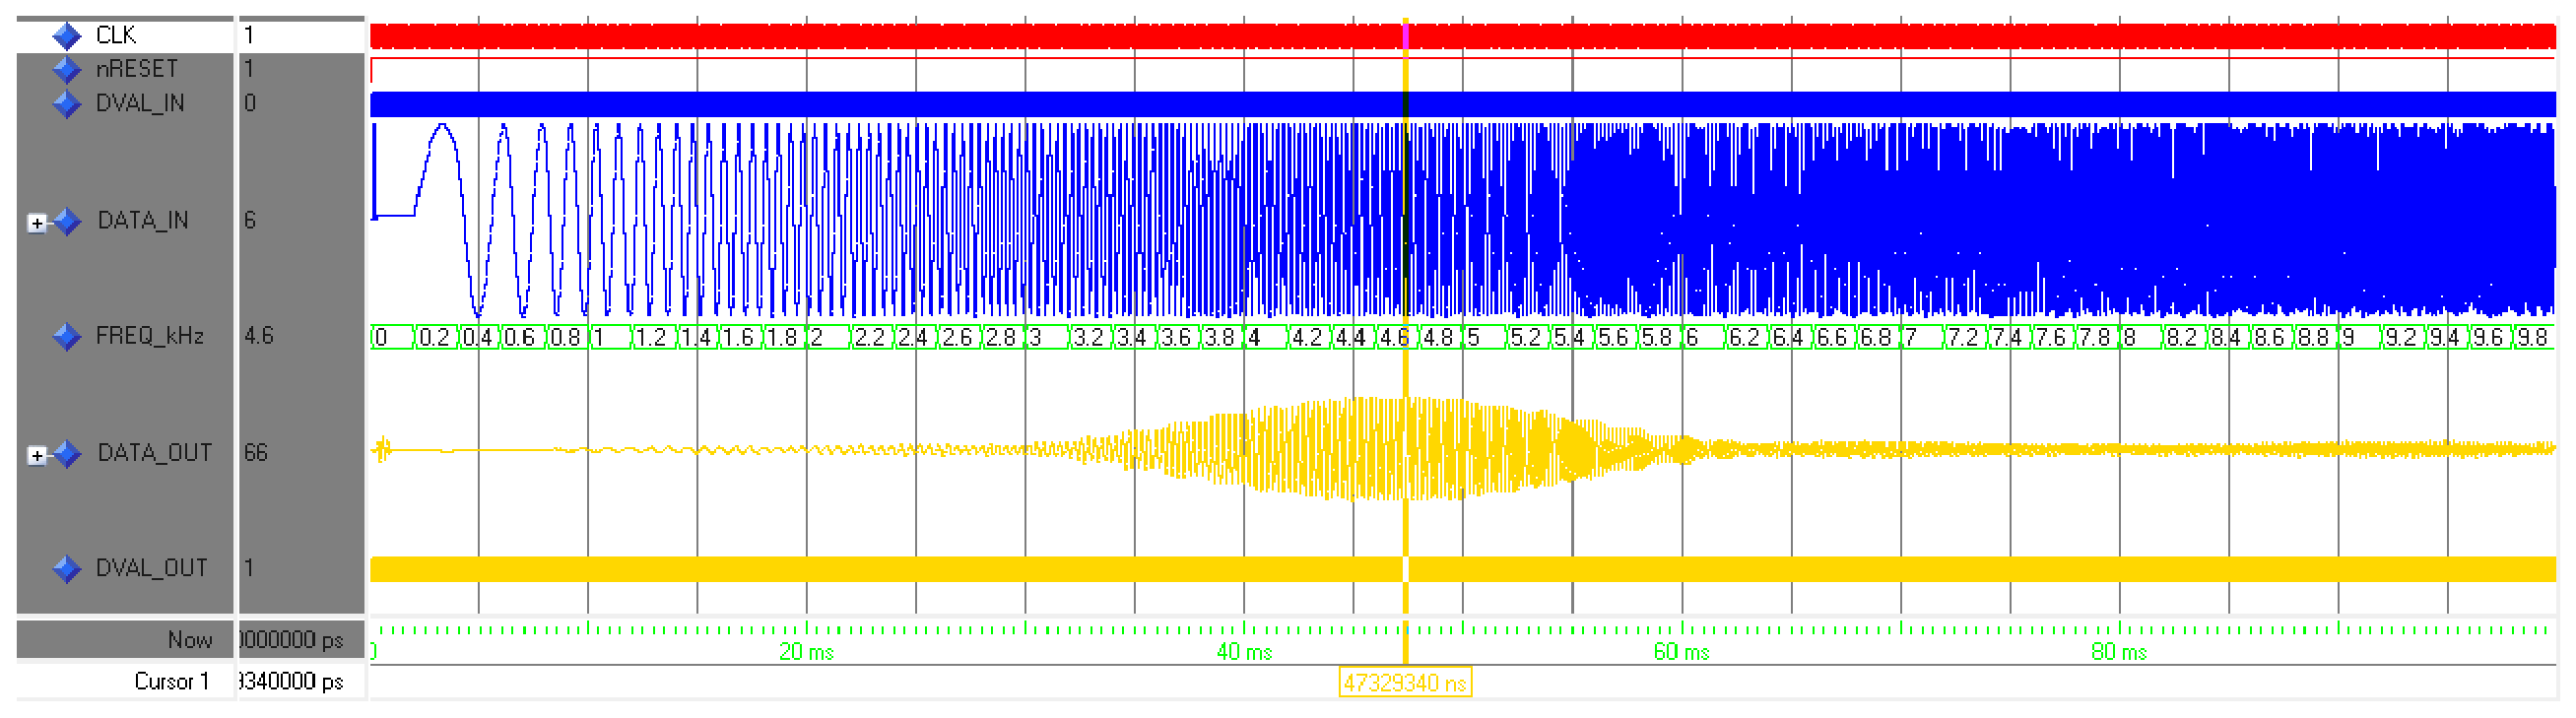
\includegraphics[width=0.8\linewidth]{bilder/filteropt}
			\end{figure}
		\end{center}
	\end{beamerboxesrounded}
\end{frame}